\section{Introduction}

\todo{Review comment: Looks inappropriate start, suggest to drop this. [DROPPED SHANNON PARAGRAPH]}

\deleted{Shanon while inventing ``digital'' showed that the communication using `symbols' is far more effective than the analog as long as the noise is under threshold. In the context of geometric algorithms, it can be interpreted as `instead of working on the final complex shape, if one is able to tokenize the shape in terms of few standard building blocks, delegate standard responsibilities to each, output would be far more deterministic'. That is the core theme of the proposed approach. It first simplifies the shape (like removal of noise, getting it below threshold), then decomposes the shape (like tokening into symbols) and then delegates midsurface computation to the decomposed blocks (like, actual communication, meaning of the symbols).}

This chapter presents an overview of the proposed system called, \replaced{\mysystemname~({\bf Mid}surface {\bf A}lgorithms for {\bf S}heet-metal-parts),}{``FSAD'' (F - Features, S - Simplification, A - Abstraction, D - Decomposition)} \replaced{for}{of} generating  a quality midsurface, \added{that is} designed and implemented in the present research work. It will assess hypotheses mentioned in Section \ref{sec:litsurvey:rquestions}. \replaced{Modules in \mysystemname~are connected in tandem and comprise of set of algorithms to carry out designated processing. The modules interact with the sheet metal feature based CAD system for exchanging and processing Brep and feature information of the CAD model. Following sections elaborate each module and their functioning.}{Following section provides an overview of \mysystemname~and the overall work-flow:}

\todo{[THINGS BELOW HAVE CHANGED A LOT, SO NOT MARKING ANY SPECIFIC CHANGES]}

\section{Overall Architecture of MidAS System}

The primary objective of the present research work is to design \deleted{and implement} a robust and automated system to generate quality midsurface by leveraging feature information. \deleted{, simplification, abstraction and decomposition.} The resultant midsurface is aimed at having minimum errors, such as gaps, overlaps, etc. and represents the input model shape. \added{Such midsurfaces can be used for variety of downstream applications such as CAE analysis of thin-walled parts, shape matching, retrieval, etc.}

\todo{Review comment: For all these modules just present on a high level, what is the input to the module, what processing happens and what is the output of the module. No mathematics, no symbols, no logic, no detailed steps. [DONE]}

%%\bigskip

	 \begin{figure} [!h]
	\centering
	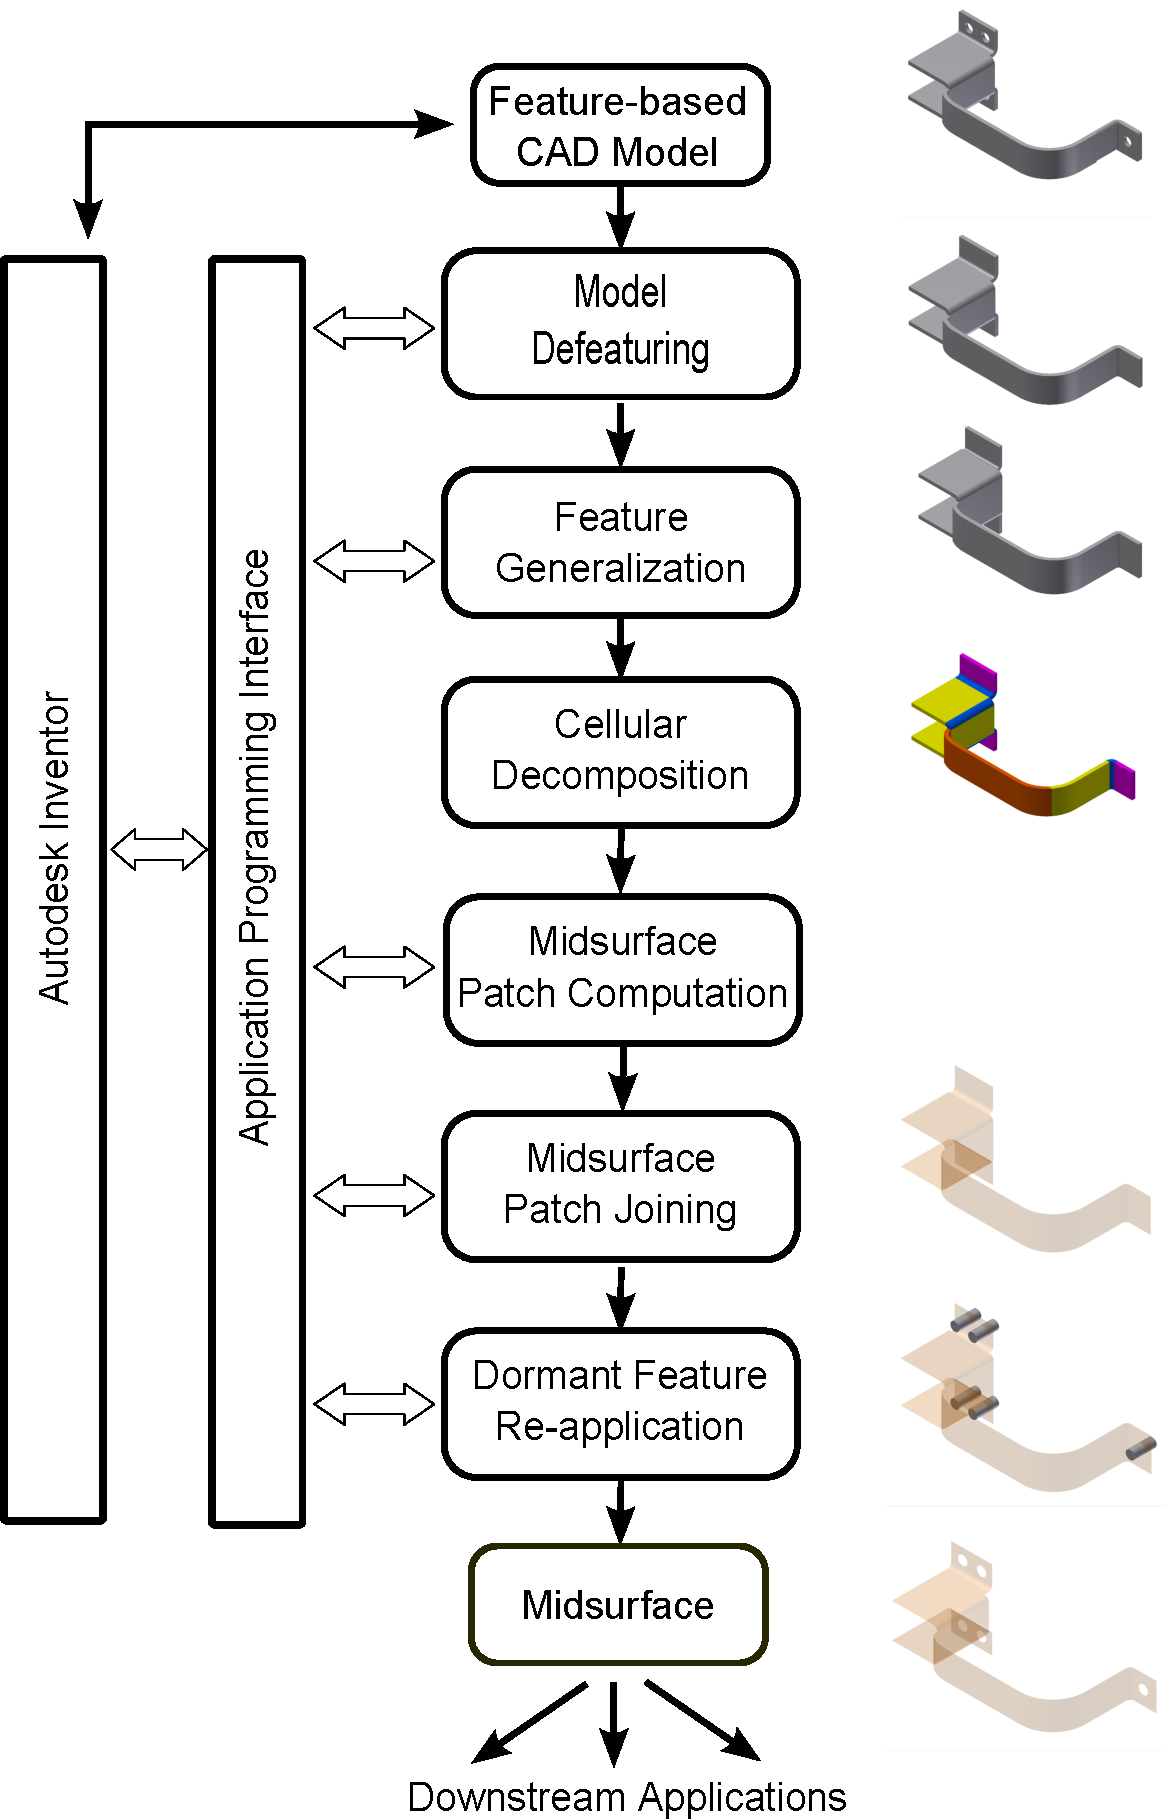
\includegraphics[width=0.62\linewidth]{images/SystemArchitecture_nolabels_7.pdf}
	%\vspace{\abovecaptionskip}
	\caption{Overall System Architecture of \mysystemname}
	\label{fig:proposal:OverallWorkflow}
	\end{figure}
	
%%\bigskip
	
Figure \ref{fig:proposal:OverallWorkflow} shows the architecture, overall work-flow and various constituent modules of the \mysystemname~system. Each module is implemented using Application Programming Interfaces (APIs)  provided by Autodesk Inventor. CAD Models shown at each stage demonstrate the transformation happening to the models. Following list elaborates each of these modules and their workings.
	
\begin{itemize}[noitemsep,topsep=2pt,parsep=2pt,partopsep=2pt]

\item \textbf{Input}:  Input to \mysystemname~is a CAD part model which is built by using a variety of sheet metal features. The model is represented as a feature history tree.

\item \textbf{Model Defeaturing}: This module defeatures the input CAD model by removing irrelevant features. The criterion for deciding relevance is based on newly devised approaches based on sheet metal feature's taxonomy and remnant feature volumes. Apart from these two approaches, in a third approach, relevant but negative features, such as Holes, Cutouts, etc. are also removed after storing their tool-feature-bodies. These features are called as Dormant features. Removal of dormant features further simplifies the model, thus making further midsurface computation stages easier. Once midsurface is computed, the stored dormant feature bodies are re-applied back so that they preserve their impression on the midsurface. Detailed approach of this module is presented in chapter \ref{ch:Defeaturing}.

\todo{[ADDED FOLLOWING PARAGRAPH AS SUGGESTED. IF IT HAS BECOME TOO BIG WE CAN PRUNE IT]}

\item \textbf{Feature Generalization}: A typical sheet metal part is modeled through a variety of sheet metal features with feature parameters. Though these features meaningfully represent the context of sheet metal domain their sheer number and variety can make the midsurface generation a complex task. \replaced{Simplifying them further will obviously make midsurface computation easier and quicker.}{still the remaining number of features could be substantial. It is obvious that simpler is the feature tree and features proper, midsurface computation is easier and quicker.} This module, with a set of algorithms transforms the actual feature tree of the model into the one represented by very basic and fundamental modeling features such as Extrude, Revolve, Sweep and Loft, along with boolean operations. \deleted{As such, Extrude, Revolve and Sweep are specialized forms of the Loft feature only. These variations, called Loft equivalents, are primarily referred in the context in which they were modeled. The output CAD model thus essentially gets represented as modeling function of {\bf A}ffine transformation, {\bf B}ooleans,  {\bf L}oft-equivalents and {\bf E}ntities, in short, known as, $\mathcal{ABLE}$ representation.}  Since such a model essentially contains only Loft-equivalent features combined with boolean operations, the complexity of the midsurface computation drastically reduces. Detailed approach and methodology of this module is presented in chapter \ref{ch:Abstraction}.

\item \textbf{Cellular Decomposition}: This module takes input a simplified and generalized feature based CAD model and decomposes it into finite number of manageable volumes called ``cells''. These cells typically represent primitive shapes of solid, each with a Loft-equivalent owner feature. The connectivity of these cells is captured in a graph based data structure.  Graph nodes are classified into midsurface patch generating nodes, called as patch nodes and midsurface patch joining nodes called as junction nodes. Cells pointed by patch nodes are called as solid cells. Cells pointed by junction nodes are called as interface cells.

\item \textbf{Midsurface Computation}: Midsurface patches are generated for each solid cell, either by offsetting the profile face or by first generating midcurve from the profile followed by lofting it. Incident midsurface patches are subsequently joined within interface cells. Details of the algorithms are presented in Chapter~\ref{ch:Midsurface}.

\todo{Review comment: Do not give these details here. Follow the pattern at previous module an provide an overview of what is input the processing and output. Essentially here we need to provide theme and not details. [REMOVED DETAILS]}

\item \textbf{Dormant Feature Re-application}: Dormant feature tool bodies are reapplied to bring back the relevant negative features onto the midsurface. 

\item \textbf{Validation}: The output midsurface is validated by newly devised approach topological validation, in which predicted topological entities of midsurface are matched with the topological entities of the actual output midsurface. Any mismatch tells the presence of errors such as missing faces, gaps, etc. This approach is only a theoretical proposal and has not been  implemented in \mysystemname.
\end{itemize}

\section{System Specifications} \label{sec:proposal:sysspecs}

\mysystemname~has been designed and developed in a modular fashion employing Object-Oriented (OO) Programming  methodology. It is implemented using OO programming languages, such as VB.Net and C\#.Net. \mysystemname~interacts with Autodesk Inventor modeler through its published APIs to query and reason the model data as well as to render the output. \deleted{The system extends the Graphical User Interfaces of Autodesk Inventor to introduce midsurface generation capabilities developed in the present research work.}

Prototype implementation has been done on Intel 64 bit processor PC.  Many of the example parts used to demonstrate the concepts, have been borrowed from GrabCAD\textsuperscript{\textregistered} site (http://www.grabcad.com).

\section{Implementation Approach} \label{sec:proposal:implementation}
Autodesk Inventor APIs were chosen for \mysystemname's implementation, because of availability of the student version for free and mature APIs over releases.  Autodesk also provides free technical support. The student version also comes with own in-built CAE module, where the output midsurface can be tested.

CAD APIs are typically used to write custom programs in various ways such as Add-Ins, External programs, etc. \mysystemname~ has built various External programs using APIs.
\todo{[REMOVED THE INVENTOR API FRAMEWORK DIAGRAM S IT WAS NOT VERY RELEVANT TO THE IMPLEMENTED SYSTEM]}
%%The Inventor API program structuring is as follows:
%%
%%	 \begin{figure} [!h]
%%	\centering
%%	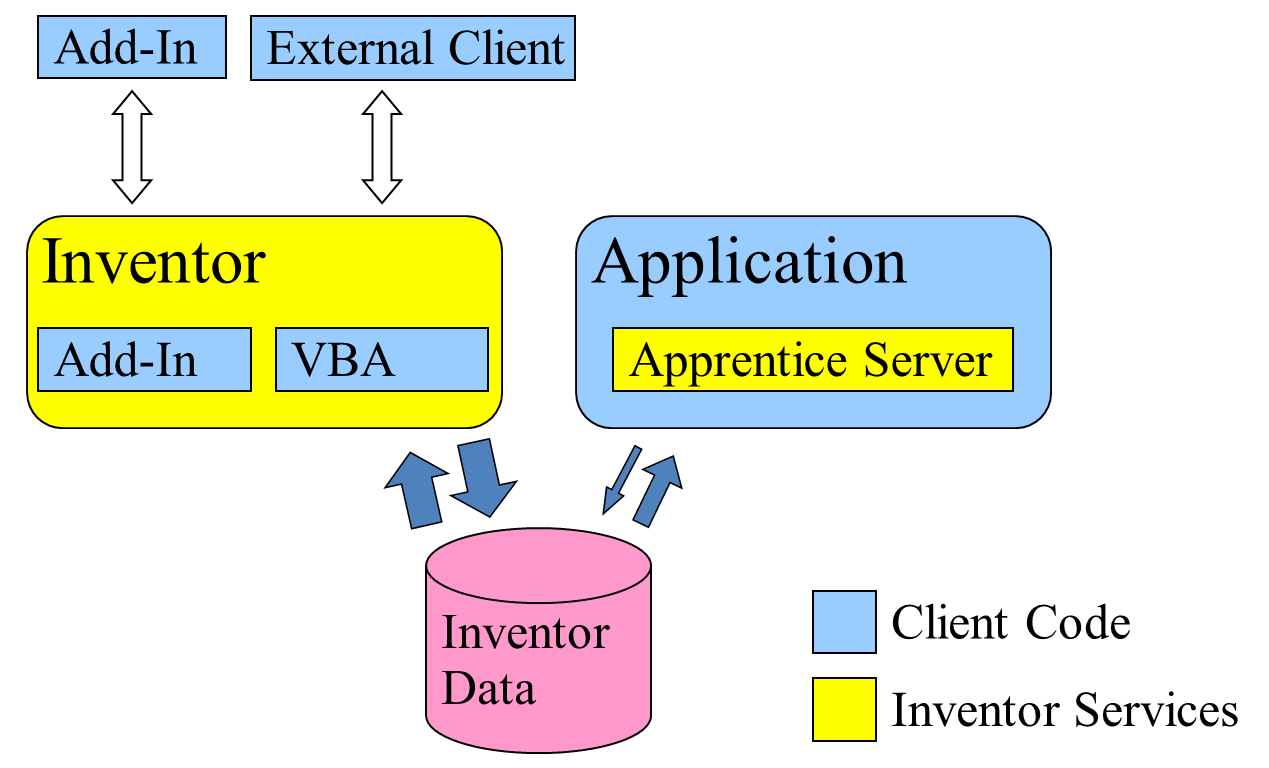
\includegraphics[width=0.9\linewidth]{images/InventorAPI}
%%	%\vspace{\abovecaptionskip}
%%	\caption{Out-of-Process/External VB.Net application }
%%	\label{fig:proposal:InventorAPI}
%%	\end{figure}
Implementation of \mysystemname~consists of neatly encapsulated software modules by using Object Oriented classes, that interact with each other through well defined interfaces. Core and internal algorithms are hidden from other classes to maintain security as well as to facilitate internal changes without disturbing the users of the classes. The modules are as follows:

\begin{itemize}
\item \textbf{Model Defeaturing}: VB.Net OO class Defeaturer encapsulates the logic of iterating over input sheet metal CAD features and removing the irrelevant ones. It exposes only the driver $Run()$ function. This function does the actual defeaturing and shows performance statistics. The defeatured model is saved with ``\_Defeatured'' extension. Tool bodies of dormant features are computed and stored to be used later for reapplication on the midsurface.
\item \textbf{Feature Generalization}: VB.Net OO class Generalizer encapsulates the logic of iterating over ``\_Defeatured' sheet metal CAD features and transforming them into generalized loft equivalents. It exposes only the driver $Run()$ function. The output generalized  $\mathcal{ABLE}$  model is saved with ``\_Able'' extension.
\item \textbf{Cellular Decomposition}: CAD model with ``\_Able'' extension is decomposed into cells, each having Loft-equivalent owner feature(s). Classes such as Graph, Node and Edge are used to populate the graph with each Node pointing to the cells. Edges are formed based on the connectivity between nodes. Nodes have attribute showing whether they are patch generating nodes or junction nodes.  The decomposed model is saved with ``\_Decomposed'' extension.
\item \textbf{Midsurface Computation}:  VB.Net program takes ``\_Decomposed'' extension CAD model and iterates over patch creating nodes of the graph. It computes midsurface by first computing the midcurve of the owner feature's sketch and then lofting it.
\item \textbf{Midcurve Computation}:  Midcurve computation program is called from patch-creation module as mentioned above, by passing sketch as input, resulting into midcurves as output.
\item \textbf{Midsurface joining}: After midsurface patches are ready, the junction nodes join the incident patches. Finally $Stitch$ function is called just to join together already well-placed midsurfaces.
\item \textbf{Dormant Re-application}: Stored dormant tool bodies are re-applied on the midsurface to pierce them through. The output midsurface is saved with ``\_Midsurface'' extension.
\end{itemize}

The output midsurface is then sent for shell meshing for CAE analysis.

%% OO methodology, modular structure, .Net architecture, Inventor external program architecture
%%
%%Following modules are developed, with clear interfaces, making them independent, easy to develop and debug.
%%\begin{itemize}
%%\item \textbf{Defeaturing}: VB.Net program takes Autodesk Inventor \textsuperscript{\textregistered} Sheet metal model and suppresses the irrelevant features.
%%\item \textbf{Abstraction}: VB.Net program takes defeatured model and converts them to Extrude/Revolve/Sweep/Loft
%%\item \textbf{Decomposition}: Splitting of abstracted model is done manually. Each sub-volume is a separate solid having either of Extrude/Revolve/Sweep/Loft as owner feature.
%%\item \textbf{Midsurface}:  VB.Net program takes decomposed solid and computes midsurface patch for each. This module then gets called in computing patches for $sCells$.
%%\item \textbf{Midcurve}:  C\#.Net program takes a polygon as input and computes the midcurve. This module gets called in the ``Midsurface'' module for patch creation.
%%\item \textbf{Midsurface joining}: VB.Net program takes decomposed solids as cells, populates a graph, classifies them into Solid Cells ($sCell$, where Midsurface pacth is generated) and Interface Cells ($iCell$, where connections happen). 
%%\end{itemize}


\section{Scope of System} \label{sec:proposal:scope}
Although Autodesk Inventor exposes most of the functionality via its APIs, it does not do so fully, due to proprietary reasons. So, all the modeling interactions that are possible in the interactive mode are not always available via APIs. This puts some restrictions on the functionality that can be developed using APIs. \deleted{Considering these restrictions the scope of the present research implementation has limited itself to certain sheet metal features and some specific modeling operations only.} It is however noted that those limitations do not anyway dilute the principles and objectives of the research. That is if the CAD modeler later provides the required capabilities through APIs, the research coverage can be extended.

\mysystemname~has been implemented to cover sheet metal feature based CAD model as input. The model is considered to be built using the library of sheet metal features provided by Autodesk Inventor's sheet metal part modeling environment.

\todo{[NEED TO REVISIT AS MANY THINGS ARE DROPED. I HAVE A LIST OF ACTUAL SHEET METAL FEATURES WE WORKED ON. SHOULD I PUT IT HERE?]}

% APIs exposed, their limitations, exact features tackeled, Autodesk specific taxonomy

\section{Overall Working of System} \label{sec:proposal:scope}

Overall working of the \mysystemname~system constitutes the following steps in sequence:
\begin{itemize}
\item The input sheet metal CAD model is either prepared afresh in Autodesk Inventor or already created model is opened in the sheet metal modeling environment.
\item Defeaturing functionally is invoked, which when run, removes all the irrelevant features and stores dormant tool bodies. 
\item Generalization functionality is invoked on the saved defeatured model. Each sheet metal feature gets converted to the corresponding Loft equivalent features, thus forming a generalized CAD model. Shape and size of the model remains as is, only the feature tree gets transformed.
\item Decomposition functionality decomposes the generalized CAD model into list of solid cells. Cells are connected to form a cellular graph. Nodes of the graph are classified as patch nodes and junction nodes. Patch nodes point to solid cells and junction nodes point to interface cells.
\item Midsurface generation module starts computing midsurface patches from solid cells and joins them in the interface cells.
\item Dormant feature tool bodies are re-applied onto the midsurface.
\item The midsurface is validated for topological and geometrical correctness.
\end{itemize}

\todo{[REMOVED THE DIAGRAM AND THE ALGORITHM]}

%%The overall algorithm for the system is:
%%
%%%%%\bigskip
%%
%%\begin{algorithm}[!h]
%%\caption{Feature based midsurface computation}
%%\label{alg_FBDMidsurf}
%%\begin{algorithmic}
%%	\REQUIRE Feature based CAD model  represented by  ($\cup_qF^3$)
%%	\STATE $\cup_wF^3 = feature\_based\_defeaturing(\cup_qF^3)$, where, $w \leq q$
%%	\STATE $\cup_wL^3 = feature\_based\_generalization(\cup_wF^3 )$
%%	\STATE $\cup_kC^3 =feature\_based\_cellular\_decomposition(\cup_wL^3)$, where, $C_i \cap C_j = 0| O_{i,j}^2$
%%	\STATE $G(a, ) = compute\_graph\_nodes(\cup_kC^3)$
%%	\STATE $G(a,b) = find\_overlaps\_generate\_edges(G(a, ))$
%%	\STATE $(sCell,iCell) = categorize\_cells(G(a,b))$
%%%	\IF{ $n_i\rightarrow edges > 2$ \& \ $n_i \rightarrow body \rightarrow is\_thin = true$ \& $O_{i,j}^2$ are adjacent} 
%%%		\STATE $type(n_i) = iCell$ 
%%%	\ELSE
%%%		\STATE $type(n_i) = sCell$
%%%	\ENDIF
%%	\FORALL{$sCell$}
%%		\STATE $\cup_aL^2 = compute\_midsurface\_patch(sCell)$ (Algorithm \ref{alg:midsurfcelljoin:MidsurfsCell})
%%	\ENDFOR
%%	\FORALL{$iCell$}
%%		\STATE $\cup_bL^2 = resolve\_interactions(iCell)$ (Algorithm \ref{alg:midsurfcelljoin:MidsurfiCell})
%%	\ENDFOR
%%	\STATE $\cup_1L^2 = (\cup_aL^2) \cup (\cup_bL^2)$
%%	\STATE $\cup_1L^2 = (\cup_1L^2) - (\cup_{dormant}L^3)$
%%	\RETURN $\cup_1L^2$
%%
%%\end{algorithmic}
%%\end{algorithm}
%%
%%%%\bigskip
%%
%%One of the screen-shots of the working system is presented below:
%%
%%%%\bigskip
%%
%%\begin{minipage}[t]{\linewidth}
%%\begin{tabular}[tb]{@{} p{0.7\linewidth} p{0.25\linewidth}@{}}
%%\adjustbox{valign=t}{
%%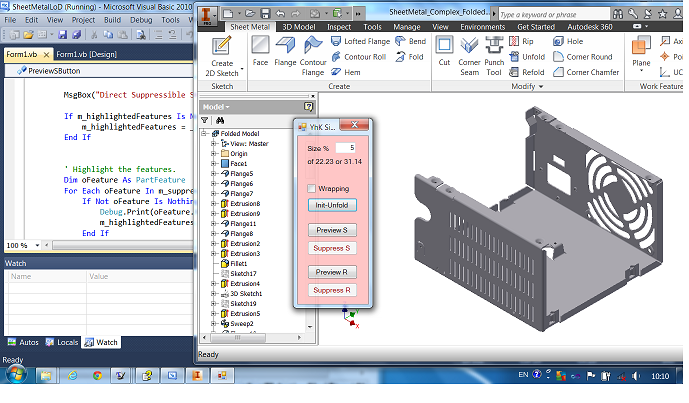
\includegraphics[width=\linewidth]{images/ImplDefeaturingProgram.png}}
%%&
%%\adjustbox{valign=t}{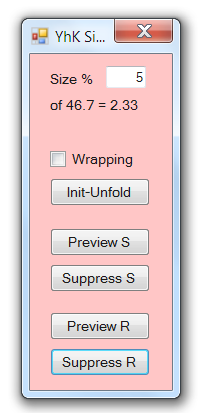
\includegraphics[width=0.8\linewidth]{images/DefeaturingDialog.png}}\\
%%\end{tabular}
%% \captionof{figure}{Screen-shot of the Defeaturing program} \label{fig:proposal:implementation}
%%\end{minipage}
%%
%%%%\bigskip

This chapter has presented an overview of the newly proposed system called \mysystemname~and its architecture. It has provided a brief review of the functional modules, the scope and the system specifications. Finally overall working of \mysystemname~has been outlined in the step-wise manner.

Following chapters present, in detail, the design and development of modules to process the CAD model by various algorithms to finally compute well-connected midsurface with a validation strategy.  
